\section{Reimplementation Strategy}
\label{sec:remplementation}

The code accompanying the original paper  is poorly written, poorly documented, and is formed of several complex and independant blocks. 
To effectively explore the core contributions of the paper, we decided to reimplement it with a more focused scope.

In our approach, we focused on reconstructing arm motion from video data, a simplification that allowed us to tackle the fundamental 
aspects of the methodology without the computational burden of full-body modeling.

\subsection{Vision Pipeline}
\label{subsec:vision_pipeline}

For 2D and 3D human pose estimation, we utilized the MediaPipe framework~\cite{lugaresi2019mediapipe}, which offers a more modern alternative 
to OpenPose. MediaPipe simplifies the vision pipeline by also replacing HMR in our usecase. An illustration of MediaPipe's inference results 
can be seen in~\cref{fig:mediapipe}. We then only used the arm joint 2D and 3D positions.

\begin{figure}
    \centering
    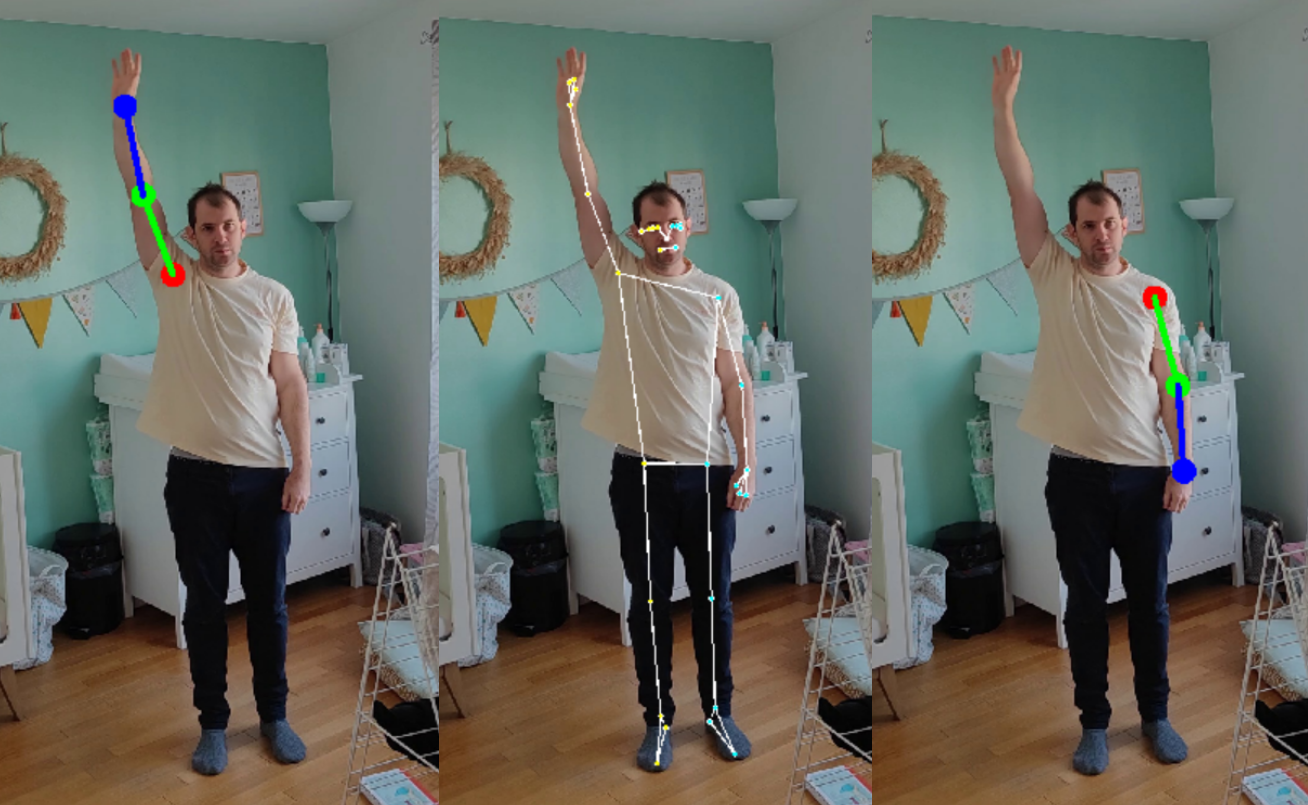
\includegraphics[width=8cm]{figures/pose_detection_mediapipe_collage.png}
    \caption{From the full body pose estimated with MediaPipe ~\cite{lugaresi2019mediapipe}, 
    we extract the arm joints for left and right arms. As a matter of homogeneous graphics,
    shoulder will always appear as red, elbow as green and wrist as blue. Upper arm will appear as green and forearm as blue.}
    \label{fig:mediapipe}
\end{figure}

Although we experimented with the contact recognizer component, we did not use it into our pipeline since we do not model contact.

\subsection{Arm Model}

We modelled the arm in Pinocchio~\cite{carpentier2019pinocchio}. The shoulder is modelized as a spherical joint, and the elbow is modelized 
as a revolute joint.

\subsection{Inverse Kinematics}
To get proper initializations to feed to the inverse dynamics optimizer, we relied on the 3D positions of the arm joints estimated by MediaPipe.
From a sequence of 3D positions of the arm joints, we used the inverse kinematics approach to estimate the joint angles.
Inverse kinematics is higly relying on the Pinocchio library ~\cite{carpentier2019pinocchio} to compute 
the Jacobian and perform forward kinematics (compute the 3D positions  $M(t)_{j}$ of the joints from the joint angles $q(t)$).
% @TODO: Add equations for IK with the 2 tasks (elbow and wrist 3D positions)

Devil is in the details, and we had to be careful about the following points:
\begin{itemize}
    \item We provide 2 tasks to the inverse kinematics solver: one for the elbow 3D position and one for the wrist 3D position. 
    Order matters, elbow comes first.
    \item The mediapipe 3D estimations are not perfect but the most nottable issue is that 
    the upper arm and the forearm lengths are not constant across time. To overcome this limitation,
    3D positions are re-scaled to match the expected nominal model arm length. 
    This arm length normalization ensures that a solution exists but on the other hand, it may introduce reprojection errors.
\end{itemize}
Although nothing grants temporal smoothness of the estimated joint angles, we recursively feed the previous solution as an initial guess to the current timestep.
This simple trick gives good results in practice (assessed qualitatively on the match between the moving arm and the video).


\subsection{Camera position}
\subsubsection{Problem formulation}
Since the upper arm can rotate in all directions and since we're not using any priors to constrain the arm motion (at the shoulder level),
moving the camera around the arm is equivalent to spinning the arm around itself. 
Our simplification unfortunately leads to a degenerate problem where the camera rotation may end up being redundant with the arm rotation.
To avoid this issue, we decided to fix the camera orientation. 
We estimate the camera 3D position $P_{\text{cam}}(t)$ 
by jointly minimizing the 2D reprojection error of joints.
$$\underset{P_{\text{cam}}(t)}{min}\sum_{j\in{\text{shoulder, elbow, wrist}}} ||K.\big[Q_{\text{cam}} | P_{\text{cam}}(t)] \vec{X}^{(j)}(t) - \vec{x}^{(j)}(t) ||$$
where
\begin{itemize}
    \item $K$ is the camera 3x3 intrinsic matrix
    \item $Q$ is the camera orientation set to identity here $I_{3}$
    \item $-P_{\text{cam}}(t)$ is the 3D camera position in the world frame (meters)
    \item $\vec{X}^{(j)}$ are the homogeneous 3D coordinates of joint $j$ (meters)
    \item $\vec{x}^{(j)}$ are the homogeneous 2D coordinates of joint $j$ in the sensor frame (pixels).
\end{itemize}

\subsubsection{Camera calibration}
To reduce the number of degrees of freedom, we always used the same camera through all our tests and 
we pre-calibrated the camera intrinsics $K$

\subsubsection{Camera pose optimization}
Each timestep can be viewed as a separate optimization problem. We can also ensure better temporal coherence
by adding a regularization term on the camera 3D position to the previous cost function $||\frac{\Delta P_{\text{cam}}}{\Delta{t}}||^2$.
We perform a first quick pass using small windows of 2 second (60 frames) to initialize the camera position sequence.
In a second pass, we optimize over the whole sequence at once.
Results are shown in \ref{fig:camera_fitting}
A rule of thumb on a i7 - 8 core CPU is that this optimizer takes roughly 1 minute to optimize the camera pose a 1 minute long video.

\begin{figure}
    \centering
    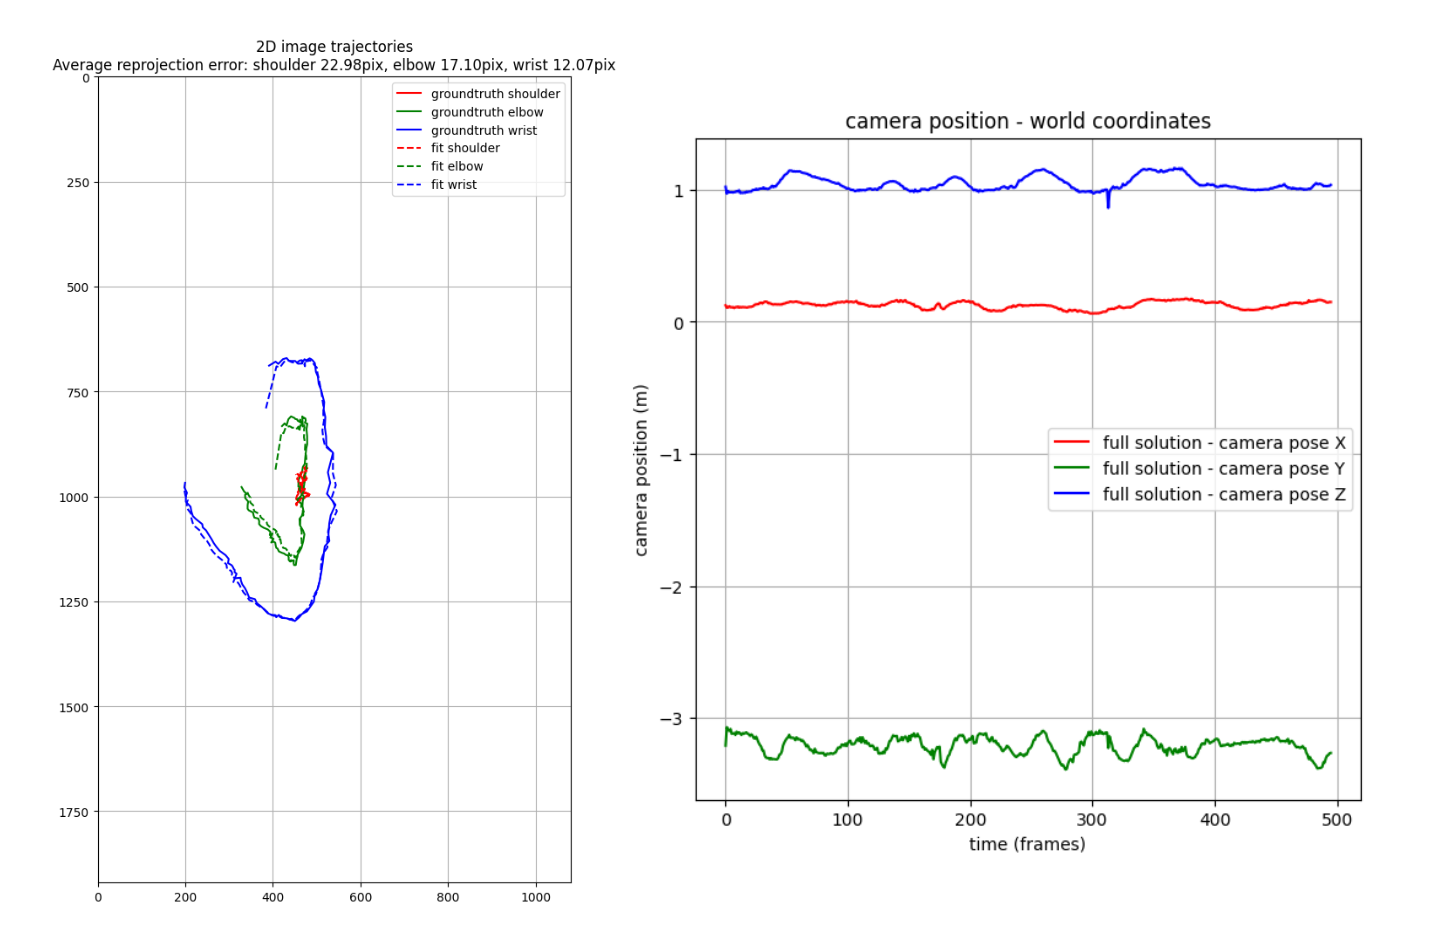
\includegraphics[width=8cm]{figures/camera_pose_fitting_collage.png}
    \caption{Left: projected arm 3D points onto the sensor after camera pose fitting - on the first 100 frames of the video (motion doing a circle with the arm). Average reprojection error reported here are computed on the 3 arm joints over the whole video.
    Right: Estimated distance from the camera to the shoulder is 3 meters wich is faithful to the real distance.}
    \label{fig:camera_fitting}
\end{figure}

\begin{figure*}
    \centering
    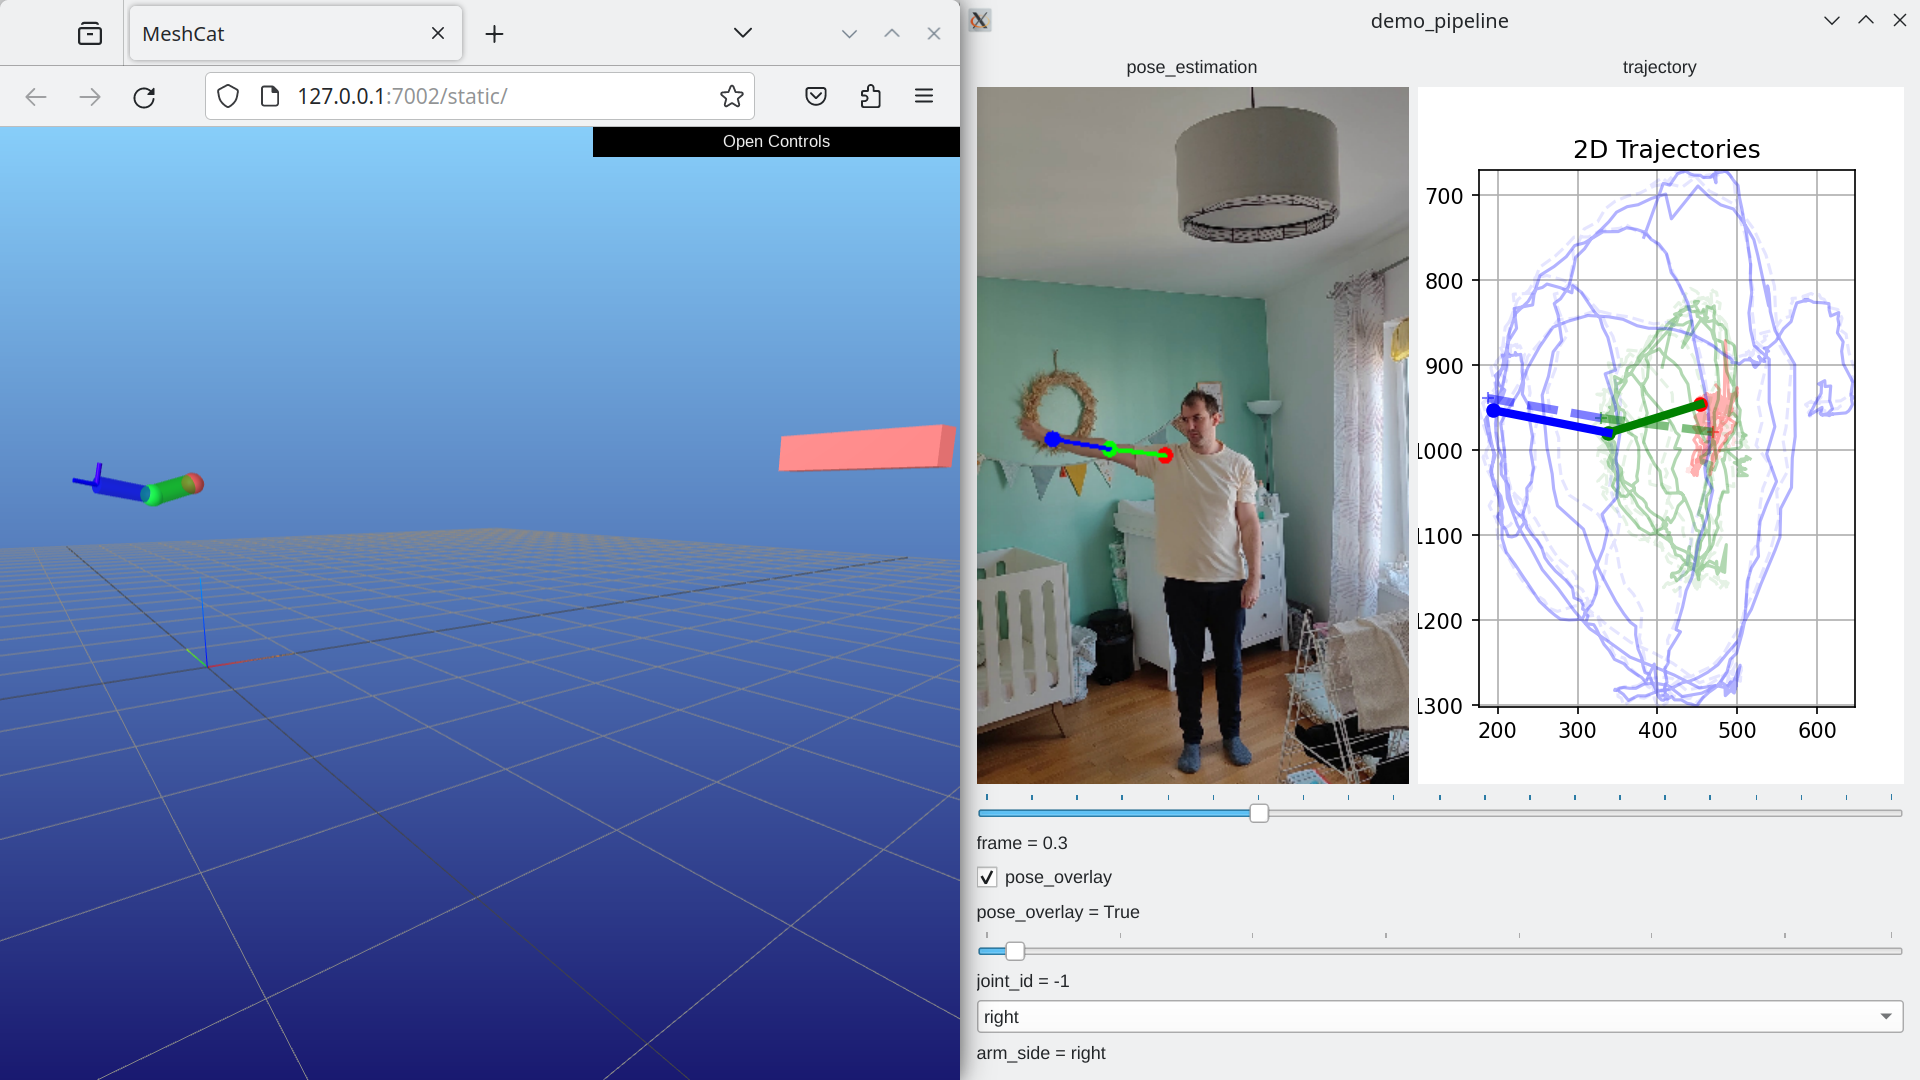
\includegraphics[width=16cm]{figures/arm_demo.png}
    \caption{Demo of the pose estimation pipeline.
    Left: Digital twin of the arm is synchronized witht the GUI. Camera is indicated in pink.
    Right: graphical user interface to select a specific frame
    and visualize the 2D joints position (dashed - right curve) aswell as the 3D reprojection of the arm (plain - right curve).}
    \label{fig:demo}
\end{figure*}

% \subsection{Initialization of the inverse dynamics optimizer}


\subsection{Inverse dynamics optimizer}

